\documentclass[a4paper,10pt]{article}
\usepackage[utf8]{inputenc}
\usepackage{graphicx}
\usepackage{amsthm,amsmath}

\title{Sarcasm detection on Reddit comments - PAKDD 2016}
%\author{Anuj Sharma}

\begin{document}

\maketitle

{\raggedright \textbf{Team Name: }DSAS}\\

{\raggedright \textbf{Team Members: }Anuj Sharma\\}

\paragraph{Summary:} A Logistic Regression (LR) estimator was built for 
detecting the level of Sarcasm in Reddit comments. The estimator was used as a 
binary classifier by means of finding an optimal threshold value beyond which a 
comment may be treated as being sarcastic.

\paragraph{Features} were extracted from the training and test dataset based on 
contents of only a single column (\emph{body}). This was done to keep the 
developed approach as generalizable as possible. Embedding of the comment words 
into vector space was carried out by extracting the following features for each 
comment:
\begin{itemize}
  \item A \emph{Bag-of-Words} (BOW) model was constructed over the entire 
training set using which comment sentences were equated to $N$ dimensional 
feature vectors. The dimensions consisted of the \emph{Term Frequency-Inverse 
Document Frequency} (TF-IDF) values of the corresponding word, where $N$ is the 
size of the vocabulary retained in the model
  \item $M$ features were added one each for $M$ Parts-of-Speech (POS) tags. 
The value was determined by the number of unique POS tags read in from the 
\emph{upenn} tagset. Each feature indicating the number of occurrences of that 
tag in the comment. Further to include interaction-events between POS tags, 
pairwise interaction terms were introduced adding ${{M}\choose{2}}$ features. 
Adding interaction terms to a regression model encapsulated relationships 
between variables which in-turn allows more hypotheses to be tested
  \item A binary feature was added indicating the presence in the comment - 
present being indicated by a 1 and absence by a 0
  \item A binary feature was added indicating the presence in the comment - 
present being indicated by a 1 and absence by a 0
  \item A feature indicating the length of the comment was added
\end{itemize}

The resulting feature set therefore consisted of $N + M + {{M}\choose{2}} + 3$ 
dimensions for each comment. The features were scaled to the range (-1.0, 1.0). 
Equation~\ref{eqn:nscale} shows how the scaled values were calculated (per 
feature) where max = $1.0$ and min = $-1.0$. 

\begin{equation} \label{eqn:nscale}
\begin{split}
X\_std = {{X - X.min()} \over {X.max() - X.min()}} \\
X\_scaled = X\_std \times (max - min) + min 
\end{split}
\end{equation}

\paragraph{Estimator} (predictive model) was then built using the training 
dataset. A Logistic Regression (LR) model was used in this work for estimating 
the probability of a comment being sarcastic.

\paragraph{Estimating a threshold} to convert the continuous predicted score 
into a binary outcome cross-validation analysis was used. The suitability of 
using LR for this task was demonstrated by carrying out a 5-fold 
cross-validation run and plotting the corresponding Receiver Operating 
Characteristic, Figure~\ref{fig:roc}, curves with the threshold varying from 0 
to 1. Subsequently 10-fold cross-validation was used to estimate a threshold 
value for which the best f-score is achieved. Both cross-validation runs were 
carried out over the entire training set.

\begin{figure}[!h]
  \centering
  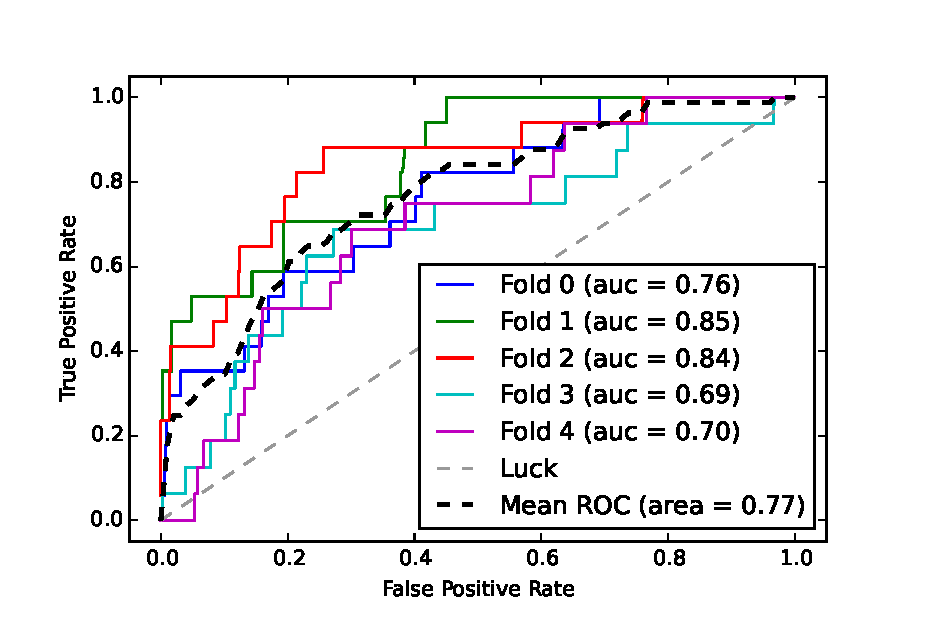
\includegraphics[width=0.5\textwidth]{roc.eps}
  \caption{Receiver Operating Characteristic curves for a 5-fold 
cross-validation analysis. The ROC curves are built with the threshold varying 
from 0 to 1.}
  \label{fig:roc} 
\end{figure}

\paragraph{Evaluation} of the LR model was carried out using 10-fold 
cross-validation over the entire dataset with the threshold value as previously 
determined. Performance of the model under 10-fold cross-validation is 
cataloged in Table~\ref{tab:perf}.

\begin{table}[!h]
\small
\centering
\par
\mbox{
\medskip
\begin{tabular}{|l|l|l|l|}
\hline
& \textbf{precision} & \textbf{recall} & \textbf{f-score}\\\hline
\textbf{Mean} & 0.53 & 0.15 & 0.23 \\\hline
\textbf{Standard Deviation} & 0.13 & 0.05 & 0.06 \\\hline
\end{tabular}
}
\caption[Performance]{Mean F-score of the LR predictive model over a 10-fold 
cross-validation analysis carried out using the training set.}
\label{tab:perf}
\medskip
\end{table}

\paragraph{Test labels} were generated using a LR predictive model built over 
the entire training set. Each comment in the test set was encoded to the 
feature space as described previously.

\end{document}
